% xivanu00 -- proj5

\documentclass[xcolor={dvipsnames}]{beamer}
\usetheme{CambridgeUS}
\usefonttheme{professionalfonts}
\setbeamertemplate{blocks}[rounded][shadow=false]
\setbeamertemplate{title page}[default][shadow=false]
\usepackage[czech]{babel}
\usepackage[utf8]{inputenc}
\usepackage[T1]{fontenc}
\usepackage{hyperref}
\usepackage{listings}
\usepackage{xcolor}
\providecommand{\uv}[1]{\quotedblbase #1\textquotedblleft}

\title{Typografie a publikování}
\subtitle{Rychlé řazení}
\author{Dmitrii Ivanushkin}
\date{\today}

\begin{document}

\begin{frame}
\titlepage
\end{frame}

\section{Úvod}
    \subsection{Řazení}
        \begin{frame}
        \begin{block}{Definice}
            \textbf{Řadicí} nebo třídicí \textbf{algoritmus} je algoritmus zajišťující uspořádání dané sady (pole, seznamu, souboru) datových záznamů do požadovaného pořadí.
        \end{block}
        \begin{exampleblock}{Příklady univerzálních druhů algoritmů}
            \begin{itemize}
                \item<1->{\textbf{Bublinkové řazení}}
                \item<2->{\textbf{Řazení haldou}}
                \item<3->{\textbf{Řazení vkládáním}}
                \item<4->{\textbf{Řazení slučováním}}
                \item<5->{\underline{\textbf{Rychlé řazení}}}
            \end{itemize}
        \end{exampleblock}
        \end{frame}
    \subsection{Motivace}
        \begin{frame}
        \begin{block}{Proč se naučit rychlé řazení?}
            \begin{itemize}
                \item<1->{\textbf{Dosahuje mnohem lepší časové složitosti O(n log n).}}
                \item<2->{\textbf{Je vhodný i pro velké datové sady s miliardami prvků.}}
                \onslide<3->{
                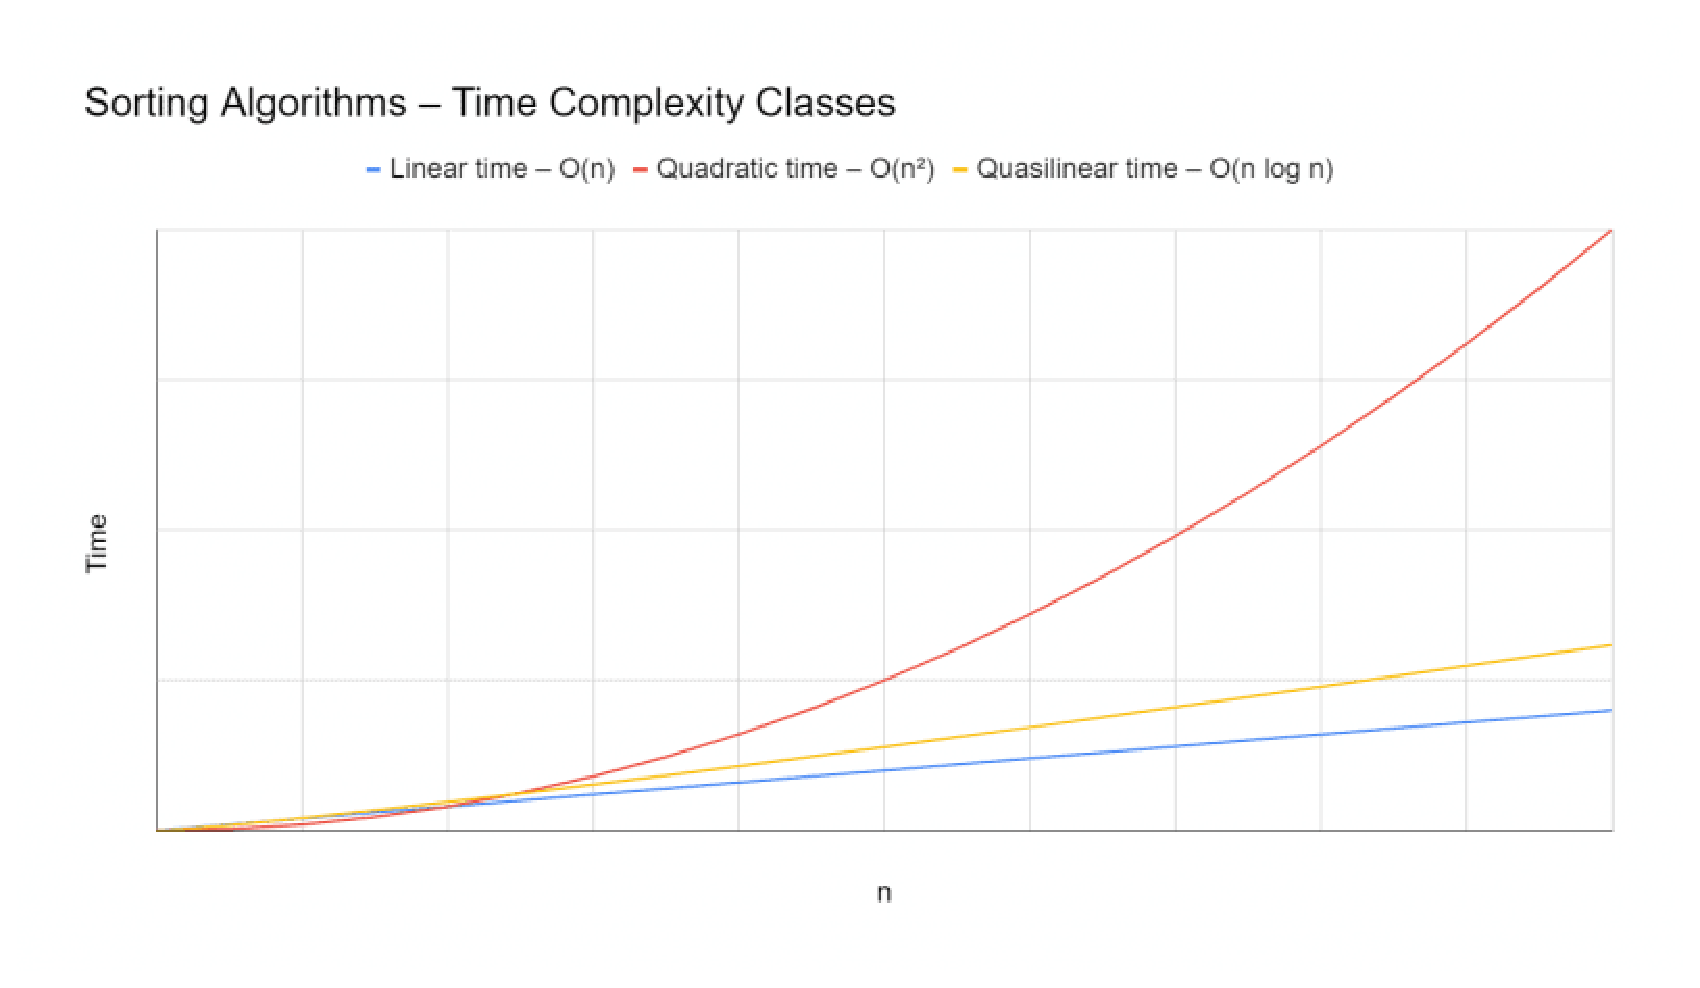
\includegraphics[scale=0.35]{pic1.eps}
                \begin{center}
                    \emph{\footnotesize{Porovnání efektivity O(n log n) časové složitosti s jinými}}
                \end{center}}
            \end{itemize}
        \end{block}
        \end{frame}
\section{Použití}
    \subsection{Algoritmus}
    \begin{frame}
    \begin{block}{Popis algoritma}
        Základní myšlenkou algoritmu rychlého řazení je rozdělení řazené posloupnosti čísel na dvě přibližně stejné části (rychlé řazení patří mezi algoritmy typu rozděl a panuj). V jedné části jsou čísla větší a ve druhé menší, než nějaká zvolená hodnota (nazývaná pivot – anglicky „střed otáčení“). Pokud je tato hodnota zvolena dobře, jsou obě části přibližně stejně velké. Pokud budou obě části samostatně seřazeny, je seřazené i celé pole. Obě části se pak rekurzivně řadí stejným postupem, což ale neznamená, že implementace musí taky použít rekurzi.
    \end{block}
    \end{frame}
    \subsection{Kroky algoritmu}
    \begin{frame}
        \begin{exampleblock}{Základní kroky algoritmu:}
        \begin{enumerate}
            \item<1->{\textbf{volba pivotu}}
            \item<2->{\textbf{přesun prvků menších než pivot před něj}}
            \item<3->{\textbf{přesun prvků větších nebo rovných pivotu za něj}}
            \item<4->{\textbf{spuštění algoritmu na část pole obsahující menší prvky}}
            \item<5->{\textbf{spuštění algoritmu na část pole obsahující větší prvky (prvky stejné jako pivot je možné přeskočit)}}
        \end{enumerate}
        \end{exampleblock}
    \end{frame}
\section{Implementace}
    \subsection{Kód v C}
    \begin{frame}[fragile]{C}
        \lstdefinestyle{c}
        {
            keywordstyle=\color{BrickRed},
            basicstyle=\ttfamily\tiny,
            breakatwhitespace=false,         
            breaklines=true,                 
            captionpos=b,                    
            keepspaces=true,                 
            numbers=none,                 
            showspaces=false,                
            showstringspaces=false,
            showtabs=false,                  
            tabsize=2,
            frame=shadowbox,
            rulesepcolor=\color{BrickRed}
        }
        \lstset{style=c}
        \begin{lstlisting}[language=C]
        void rychlerazeni(int array[], int levy_zacatek, int pravy_zacatek)
        {
        int pivot = array[(levy_zacatek + pravy_zacatek) / 2];
        int levy_index, pravy_index, pom;
        levy_index = levy_zacatek;
        pravy_index = pravy_zacatek;
        do {
            while (array[levy_index] < pivot && levy_index < pravy_zacatek) 
                levy_index++;
            while (array[pravy_index] > pivot && pravy_index > levy_zacatek) 
                pravy_index--;
                
            if (levy_index <= pravy_index) {
                pom = array[levy_index];
                array[levy_index++] = array[pravy_index];
                array[pravy_index--] = pom;
            }
        } while (levy_index < pravy_index);

        if (pravy_index > levy_zacatek) rychlerazeni(array, levy_zacatek, pravy_index);
        if (levy_index < pravy_zacatek) rychlerazeni(array, levy_index, pravy_zacatek);
        }
        \end{lstlisting}
    \end{frame}
\section{Literatura}
    \begin{frame}{Použité zdroje}
        \begin{thebibliography}{99}
        \bibitem{1} J. Rychlík. Programovací techniky. 2., upravené vyd. České Budějovice: KOPP, 1995. 188 s. ISBN 80-85828-05-7. Kapitola 6 – Řazení.
        \bibitem{2} S. Woltmann. Happy coders. [online], [vid. 2022-05-05]. \url{www.happycoders.eu/algorithms/sorting-algorithms/}
        \bibitem{3} Wikipedia. [online], [vid. 2022-05-05].
        \url{https://en.wikipedia.org/wiki/Quicksort}
        \bibitem{4} V. Hordejčuk. Quick sort (rychlé řazení). [online], [vid. 2022-05-05].
        \url{http://voho.eu/wiki/quick-sort/}
        \end{thebibliography}
    \end{frame}
 
\end{document}
